\section{Introduction}
This section provides an overview of the fundamental principles underlying the experience.

	\subsection{Feedback}
		A feedback loop is created when all or some portion of the output is fed back to the input. 
		Negative feedback occurs when the fed-back output signal has a relative phase of $\pi$ with respect to the input signal, 
		while positive feedback occurs when the signals are in phase.
	
	\subsection{Operational amplifier}
		An operational amplifier, often abbreviated as op-amp, is a voltage-controlled voltage generator.
		The op-amp's primary function is to amplify the difference in voltage between its two input terminals, usually labeled as the inverting input (-) and the non-inverting input (+). 
		It has a high input impedance, meaning it draws very little current from the input sources, and a low output impedance, enabling it to drive other circuit components effectively. 
		In its ideal form, an op-amp has infinite voltage gain, however, real-world op-amps have limitations due to factors like power supply voltage, noise, and frequency response. 
		Op-amps are often used in circuits with negative feedback.
	
	\subsection{Virtual ground}
		The concept of a virtual ground is a fundamental aspect of negative feedback operational amplifier (op-amp) circuits. 
		In these circuits, a virtual ground is created at the inverting input terminal of the op-amp, even though it is not physically connected to the ground reference. 
		This virtual ground serves as a reference point for analyzing and designing circuits, allowing for simplified calculations and intuitive understanding.
		In fact, negative feedback attempts to drive the inverting input to a voltage that matches the non-inverting input, which can result in $V^+ - V^- = \SI{0}{\volt}$ and, consequently, $I^+ = I^-$.
		An op-amp is a voltage-controlled voltage generator, so it does not absorb current at the input (behaves like an open circuit), therefore $I^+ = I^- = \SI{0}{\ampere}$. 

	\subsection{Differentiator circuit}
		The differentiator circuit's functionality is firmly grounded in the mathematical concept of differentiation, a fundamental calculus concept.
		Analogous to how differentiation calculates the rate of change of a mathematical function concerning its independent variable, 
		the differentiator circuit accentuates swift variations in input signal amplitude. \\\\
		The differentiator circuit's design involves the integration of passive and active electronic components:
		capacitors and resistors play pivotal roles in shaping the circuit's frequency response, allowing it to differentiate signal components with varying frequencies, 
		while the operational amplifier is employed to achieve high gain and accurate differentiation by ensuring that the inverting input adheres to a voltage level analogous to ground potential. \\
		The schematic diagram of the differentiator circuit is illustrated in Figure \ref{fig:differentiator_circuit}. \\\\
		\begin{figure}[H]
		    \centering
		    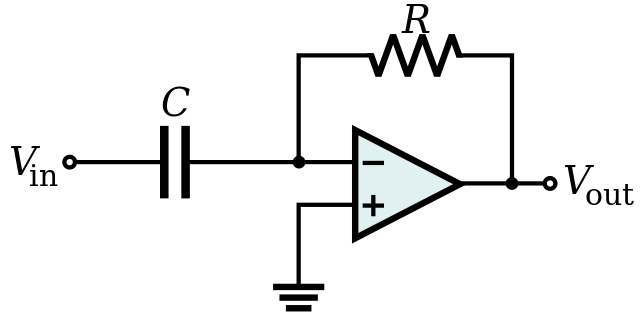
\includegraphics[width=0.4\textwidth]{figures/differentiator/circuit.png}
		    \caption{Differentiator circuit schematic.}
		    \label{fig:differentiator_circuit}
		\end{figure}
		\noindent 
		Applying the Kirchhoff's circuit laws at the op-amp's inverting input terminal, which is held at ground potential due to the virtual ground concept, 
		it is possible to establish that the current flowing in the capacitor is equal to the current through the resistor, $i_C(t) = i_R(t), \forall t$, and further more: 
		$$ C \cdot \frac{d}{dt}(V_{in}(t) - V^-) = \frac{V^- - V_{out}(t)}{R} $$
		Remembering that $V^- = \SI{0}{\volt}$, by solving the equation for $V_{out}$, 
		it is shown that the output of the differentiator circuit is proportional to the rate of change of the input signal with respect to time: $$ V_{out}(t) = - RC \cdot \frac{d}{dt}V_{in}(t) $$
		
	\subsection{Integrator circuit}
		The integrator circuit can be easily obtained from a differentiator circuit by simply swapping the resistor and the capacitor. 
		The schematic diagram of the circuit is illustrated in Figure \ref{fig:integrator_circuit}. \\\\
		Similar to the approach taken with the differentiator circuit, Kirchhoff's circuit laws can be employed at the virtual ground node to obtain the equation that characterizes the integrator circuit's behavior: $$ \frac{V_{in}(t)}{R} = - C \cdot \frac{d}{dt}V_{out}(t) \quad \Longrightarrow \quad V_{out}(t) = - \frac{1}{RC} \cdot \int_{\SI{0}{\second}}^t V_{in}(\tau)d\tau + V(\SI{0}{\second}) $$
		Notably, the output voltage is proportional to the integral of the input voltage over time, with adjustments related to the time constant and the initial conditions of the circuit. \\
		The term $V(\SI{0}{\second})$ represents the initial condition of the output voltage at $t=\SI{0}{\second}$ and plays a pivotal role in shaping the behavior of the circuit, as it introduces an offset or a foundational voltage level to the integrated output signal. 
		This offset can serve as a calibration factor, facilitating the alignment of the output signal with a desired reference level. \\
		For instance, in cases where the initial measurements demonstrated an unexpected shift, it became imperative to introduce a robust resistor ($R=\SI{0.98}{\mega\ohm}$) to the circuit. 
		This strategic inclusion was necessary to rectify the observed shifts in measurements and to achieve the desired circuit response. 
		The high-value resistor played a crucial role in mitigating these deviations and aligning the measurements with the intended outcomes.
		\begin{figure}[H]
		    \centering
		    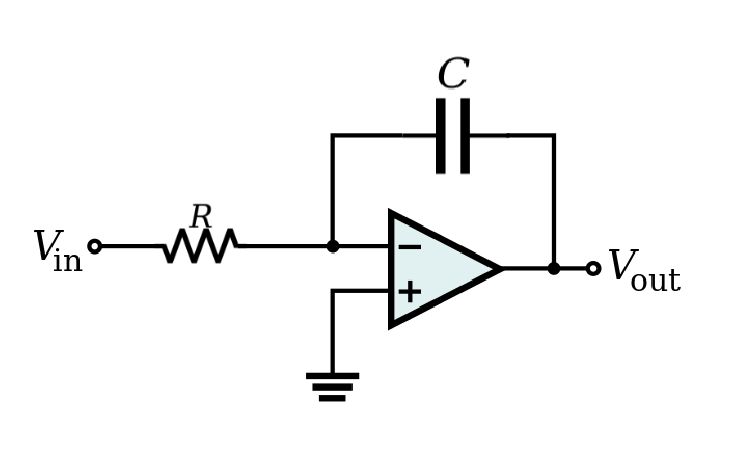
\includegraphics[width=0.5\textwidth]{figures/integrator/circuit.png}
		    \caption{integrator circuit schematic.}
		    \label{fig:integrator_circuit}
		\end{figure}
